\documentclass[journal]{IEEEtran}

\usepackage{amsmath,amssymb,amsfonts}
\usepackage{algorithmic}
\usepackage{algorithm}
\usepackage{graphicx}
\usepackage{textcomp}
\usepackage{xcolor}
\usepackage{booktabs}
\usepackage{multirow}
\usepackage{subcaption}
\usepackage{tikz}
\usepackage{pgfplots}
\usepackage{hyperref}
\usepackage{cleveref}
\usepackage{siunitx}
\usepackage[pagewise,mathlines]{lineno}
\renewcommand\linenumberfont{\normalfont\tiny\sffamily\color{gray}}\setlength{\linenumbersep}{4pt}

\usetikzlibrary{shapes.geometric, arrows.meta, positioning, fit, backgrounds, calc, patterns}
\pgfplotsset{compat=1.18}


\usepackage[scaled=0.92]{helvet}
\pgfplotsset{every axis/.append style={font=\sffamily}}
\tikzset{every picture/.style={/utils/exec=\sffamily}}

\hypersetup{
    colorlinks=true,
    linkcolor=blue,
    citecolor=blue,
    urlcolor=blue,
    pdftitle={Unsupervised deep learning for wavelength selection in ME-HSI},
    pdfauthor={Narek Meloyan},
}

\clubpenalty=10000
\widowpenalty=10000
\displaywidowpenalty=10000
\brokenpenalty=10000

\newcommand{\lambdaex}{\lambda_{\text{ex}}}
\newcommand{\lambdaem}{\lambda_{\text{em}}}
\newcommand{\R}{\mathbb{R}}
\newcommand{\vect}[1]{\mathbf{#1}}
\newcommand{\mat}[1]{\mathbf{#1}}

\begin{document}

\title{Unsupervised Deep Learning for Wavelength Selection in Multi-Excitation Fluorescence Imaging}

\author{\IEEEauthorblockN{Narek Meloyan\textsuperscript{1,2}, Narine Sarvazyan\textsuperscript{1,2,3}}
\\
\IEEEauthorblockA{\textsuperscript{1}American University of Armenia, Yerevan, Armenia\\
\textsuperscript{2}L.A. Orbeli Institute of Physiology NAS RA, Yerevan, Armenia\\
\textsuperscript{3}George Washington University, Washington, DC, USA\\
Email: narek\_meloyan@edu.aua.am, phynas@gwu.edu}}

\maketitle
\linenumbers

\begin{abstract}
Conventional Hyperspectral Imaging (HSI) acquires reflectance, emission, or excitation profiles at each pixel.
Emission-based HSI can be expanded into a fourth dimension by varying the excitation wavelength, improving discrimination of materials that contain mixed fluorophores.
Multi-excitation HSI (ME-HSI) thus forms a 4D dataset spanning two spatial and two spectral dimensions (emission and excitation wavelengths).
Processing ME-HSI datasets is challenging: the many spectral layers per pixel introduce redundancy and computational burden, and band selection methods developed for 3D HSI fail to capture the nonlinear cross-excitation correlations present in ME-HSI data.
To address this gap, a deep learning framework was developed comprising three stages: (1) a 3D convolutional autoencoder with parallel excitation branches that learns a unified latent representation, (2) a perturbation-based attribution method that traces reconstruction sensitivity to individual excitation-emission wavelength pairs, and (3) Maximum Marginal Relevance (MMR) selection that balances informativeness with spectral diversity.
Evaluated on lichen samples with four ground-truth classes, the framework exceeded the full-spectrum baseline while using only 9 of 192 bands (95\% data reduction).
Applied without retuning to a chemically distinct collagen sponge dataset, it again exceeded the baseline using a small fraction of the bands.
The proposed approach allows to mitigate the computational and hardware challenges of ME-HSI by dramatically decreasing acquisition complexity while boosting its discriminative power.
\end{abstract}

\begin{IEEEkeywords}
Wavelength selection, convolutional autoencoder, perturbation analysis, spectral band selection, fluorescence imaging.
\end{IEEEkeywords}

\section{Introduction}
\label{sec:introduction}

\IEEEPARstart{H}{yperspectral} imaging has become an established technology for remote sensing, material characterization, and biomedical analysis, capturing reflected or emitted light across hundreds of contiguous wavelength bands, exceeding the discriminative capabilities of RGB or multispectral data~\cite{plaza2009recent,bioucas2013hyperspectral,hong2024spectralgpt,tran2026medical}.
Recent applications range from Earth observation---for example the detection of photovoltaic power plants from satellite and airborne sensors~\cite{joerges2023photovoltaic} and the unsupervised unmixing of oceanic scenes affected by spectral variability and adjacency effects~\cite{deville2023oceanic}---to laboratory and clinical imaging, where the measured signal is increasingly fluorescence rather than reflectance.
In all of these settings the number of acquired bands is a recurring cost, which motivates the selection of a small informative subset.
While reflectance-based HSI measures how materials scatter
incident light, fluorescence-based HSI traditionally captures the emission spectra produced when materials absorb ultraviolet or visible light and re-emit photons at longer wavelengths.
This fluorescence response encodes molecular-level information about chromophores, enabling discrimination of materials that appear identical under reflectance imaging but possess distinct fluorescent signatures~\cite{muselimyan2016,gil2017}.

The multi-excitation HSI (ME-HSI) approach combines
acquisition of emission profiles with stepwise changes in the
wavelength of illuminating light, yielding a four-dimensional data structure spanning two spatial $(x, y)$, and two spectral dimensions, namely emission $\lambda_{\text{em}}$, and excitation wavelengths $\lambda_{\text{ex}}$.
This yields a simplified version of the excitation-emission matrix (EEM) for each spatial pixel, a comprehensive fluorescence fingerprint that has proven valuable for a variety of different applications~\cite{lakowicz2006principles,swift2018}.

The discriminative power of ME-HSI comes at a computational cost.
An example acquisition with $N_{\text{ex}} = 8$ excitation wavelengths and $N_{\text{em}} = 24$ emission bands per excitation yields 192 data points per pixel, which for a megapixel image (e.g., $1040 \times 925$ pixels) translates to over 184 million data points per ME-HSI dataset.
Not all of these excitation-emission combinations carry discriminative information: spectral overlap between fluorophores, detector noise in low-signal regions, and physical constraints such as Rayleigh scattering near the excitation wavelength introduce redundancy.
The fundamental question thus becomes: \emph{which excitation-emission wavelength pairs actually matter for discriminating materials of interest?}
Answering this question has direct implications for:
(i)~sensor design, reducing the number of required LEDs, filters, and detector channels;
(ii)~real-time processing, enabling faster classification; and
(iii)~system deployment, decreasing power consumption and data transmission requirements.

The challenge of identifying informative spectral bands has been extensively studied for conventional 3D HSI~\cite{sun2019hyperspectral,rasti2020featureextraction,jia2020survey,asfour2018,guan2018}, with approaches spanning filter-based methods (variance, entropy), wrapper methods (sequential forward selection, genetic algorithms), and embedded methods (sparse regression, attention mechanisms)~\cite{martinez2006comparison,chang2000constrained,pudil1994floating,pal2010feature,tibshirani1996regression,lorenzo2020attention}.
However, these approaches have notable limitations when applied to ME-HSI: filter-based methods lack task relevance, wrapper methods suffer from prohibitive computational cost when the search space is large, and embedded methods require labeled training data.
Importantly, the vast majority of these methods treat each spectral band independently, assuming a 3D data structure of $(x, y, \lambda)$ where bands can be selected without considering their relationship to excitation wavelengths.
For ME-HSI data, the information lies in specific excitation-emission \emph{combinations} and the nonlinear correlations between excitations may include important discriminative patterns.
Therefore, methods that explicitly model the joint spectral-spatial structures are needed.
To the best of our knowledge, no existing band selection method addresses this 4D structure directly.

Deep learning offers a principled approach to learning nonlinear representations from high-dimensional data without requiring explicit feature engineering~\cite{lecun2015deep}.
Autoencoders, which learn compressed representations by training a network to reconstruct its inputs, provide an unsupervised mechanism for identifying the essential structure in data~\cite{hinton2006reducing,bengio2013representation}.
An autoencoder trained on ME-HSI data must encode the information necessary to reconstruct all excitation-emission combinations; analyzing what the autoencoder has learned, specifically probing the sensitivity of reconstruction to perturbations in the latent space, enables attribution of importance to individual wavelengths without requiring class labels.
This insight connects representation learning to feature selection: the autoencoder identifies important features implicitly through compression, and perturbation analysis makes this implicit knowledge explicit.

This paper presents an unsupervised deep learning framework for wavelength selection in ME-HSI datasets, combining a 3D convolutional autoencoder (CAE) with parallel excitation branches, perturbation-based attribution, and Maximum Marginal Relevance (MMR) selection~\cite{carbonell1998use}.
The framework requires no class labels and produces ordered wavelength rankings at any desired reduction level; the methodology is detailed in Section~\ref{sec:methodology}.
The framework is evaluated on two independent fluorescence datasets (lichen samples and collagen sponges) that differ in their excitation grids, valid band counts, and class structures, providing complementary tests of the same approach.
To the best of our knowledge, this represents the first deep learning approach for wavelength selection in 4D ME-HSI data.
\section{Related Work}
\label{sec:related_work}

This section reviews prior work in four areas relevant to the present framework: hyperspectral imaging systems and data characteristics, band selection methods for hyperspectral data, deep learning approaches for spectral analysis, and explainability methods for feature attribution.
The four parts are ordered from the data to the method: the modality and its 4D structure motivate the problem (Section~\ref{sec:related_hsi}), existing band selection methods define the gap (Section~\ref{sec:related_band}), deep representation learning (Section~\ref{sec:related_dl}) and perturbation-based attribution (Section~\ref{sec:related_explain}) supply the two tools that the framework combines, and the final part positions the framework against them (Section~\ref{sec:related_summary}).

\subsection{Multi-Excitation Hyperspectral Imaging Systems}
\label{sec:related_hsi}

Hyperspectral imaging systems have evolved from early pushbroom scanners requiring platform motion~\cite{goetz1985imaging} to contemporary snapshot sensors capable of real-time acquisition~\cite{hagen2013review}.
While reflectance-based hyperspectral imaging remains dominant for remote sensing applications, fluorescence hyperspectral imaging has gained traction in laboratory and close-range settings where controlled excitation is feasible~\cite{mishra2017close}.
The extension to multiple excitation wavelengths---yielding the EEM structure that characterizes ME-HSI---was pioneered in analytical chemistry for fluorescence spectroscopy of solutions~\cite{murphy2013fluorescence} and has been adapted for imaging applications where spatially resolved EEM data provides additional discrimination power~\cite{lavine2001exploratory}.
Such systems have proven particularly valuable for biological specimens, including lichens and plant tissues, where autofluorescence signatures encode information about molecular composition that reflectance imaging cannot capture~\cite{croce2019autofluorescence}.

The 4D data structure of ME-HSI presents unique challenges.
Unlike 3D hyperspectral cubes where spectral bands sample a single physical phenomenon (reflectance or emission at fixed excitation), ME-HSI data exhibits complex cross-excitation correlations arising from energy transfer between fluorophores, concentration-dependent quenching, and overlapping emission spectra~\cite{lakowicz2006principles}.
Additionally, Rayleigh and Raman scattering at wavelengths near the excitation produce artifacts that must be removed, resulting in variable numbers of valid emission bands per excitation~\cite{murphy2013fluorescence}.
While hardware advances have made 4D acquisition practical, analytical methods for handling the resulting data dimensionality have lagged behind~\cite{mishra2017close}.

\subsection{Band Selection for Hyperspectral Data}
\label{sec:related_band}

Band selection methods aim to identify a subset of spectral bands that retain discriminative information while reducing dimensionality~\cite{sun2019hyperspectral,rasti2020featureextraction}.
These methods are typically categorized as filter, wrapper, or embedded approaches; the specific contribution of each family, and its limitation for ME-HSI data, are summarized in turn.

\textbf{Filter methods} rank bands based on statistical properties computed without reference to any downstream task.
Variance-based selection prioritizes bands with high variance across samples~\cite{chang2000constrained}, entropy-based methods favor bands with maximum information content~\cite{guo2006band}, and correlation-based approaches remove redundant bands that are highly correlated with others~\cite{martinez2006comparison}.
While computationally efficient, filter methods lack any notion of discriminative value---a band with high variance may capture noise rather than meaningful variation.
Moreover, they treat bands independently, ignoring the joint information captured by band combinations.

\textbf{Wrapper methods} evaluate band subsets based on the performance of a classifier trained on the selected features.
Sequential forward selection (SFS) greedily adds bands that most improve classification accuracy~\cite{pudil1994floating}, while genetic algorithms and particle swarm optimization explore the combinatorial search space more globally~\cite{pal2010feature}.
These methods can identify task-relevant bands but suffer from computational cost that grows combinatorially with the number of bands.
For a 192-band ME-HSI dataset, exhaustive evaluation of all possible subsets is intractable.

\textbf{Embedded methods} integrate band selection into model training.
Sparse regression (LASSO) induces feature selection through $L_1$ regularization~\cite{tibshirani1996regression}, and attention mechanisms in neural networks trained for classification learn to weight input bands~\cite{lorenzo2020attention}.
While elegant, these approaches typically require labeled training data, limiting their applicability when ground truth is scarce or expensive to obtain.

\textbf{Unsupervised deep methods} learn band weights jointly with a reconstruction network and read the selection off the learned weights, as in BS-Nets~\cite{cai2020bsnets}.
Their contribution is label-free, end-to-end selection; their limitation is that a single attention layer over a single spectral axis presumes one rectangular cube, and that the selection is fixed at training time.

Critically, nearly all existing band selection methods assume a 3D data structure where bands can be evaluated independently.
For ME-HSI, where information lies in excitation-emission \emph{pairs} and cross-excitation patterns may be discriminative, methods that explicitly model the 4D structure are needed.
Recent work on tensor decomposition for EEM data~\cite{murphy2013fluorescence} and multi-way analysis~\cite{bro1997parafac} addresses spectroscopic rather than imaging data.
The present framework bridges this gap by extending deep learning band selection to the 4D imaging case.

\subsection{Deep Learning for Hyperspectral Analysis}
\label{sec:related_dl}

Deep learning has substantially advanced hyperspectral image analysis, with convolutional neural networks achieving state-of-the-art results in classification, segmentation, and anomaly detection~\cite{li2019deep,paoletti2019deep}.
Early approaches applied 2D CNNs to spectral vectors treated as 1D signals~\cite{hu2015deep}, while subsequent work exploited spatial context through 3D convolutions that jointly process spatial and spectral dimensions~\cite{chen2016deep}.
Architectures such as spectral-spatial residual networks~\cite{zhong2017spectral} and HybridSN~\cite{roy2020hybridsn} combine 3D convolutions for spectral-spatial feature extraction with 2D convolutions for spatial refinement, achieving classification accuracies exceeding 95\% on standard benchmarks.

For unsupervised analysis, autoencoders have been applied to hyperspectral data for compression~\cite{chen2014deep}, denoising~\cite{vincent2008extracting}, and feature extraction~\cite{mou2017unsupervised}.
Variational autoencoders (VAEs) provide probabilistic latent representations that enable uncertainty quantification~\cite{kingma2013auto}, while sparse autoencoders encourage disentangled features through sparsity constraints~\cite{ng2011sparse}.
Stacked convolutional autoencoders~\cite{masci2011stacked} have demonstrated the ability to learn hierarchical features from spectral data without supervision.
These works focus on learning representations for downstream classification; in contrast, the present framework uses the learned representation as the basis for wavelength attribution.

Most deep learning approaches for hyperspectral data assume a 3D input structure.
While 3D convolutions naturally extend to 4D data by adding an excitation dimension, the variable number of emission bands per excitation after Rayleigh cutoff complicates a monolithic architecture.
The parallel-branch design introduced here addresses this limitation, enabling end-to-end learning on 4D ME-HSI data with heterogeneous spectral dimensions.

\subsection{Explainability and Attribution Methods}
\label{sec:related_explain}

Explaining neural network predictions has become crucial for scientific applications where understanding \emph{why} a model makes decisions is as important as accuracy~\cite{gilpin2018explaining}.
Post-hoc explanation methods include saliency maps that compute gradients of outputs with respect to inputs~\cite{simonyan2014deep}, Grad-CAM that localizes class-discriminative regions~\cite{selvaraju2017grad}, LIME that fits local linear models~\cite{ribeiro2016should}, and SHAP that provides game-theoretic feature attributions~\cite{lundberg2017unified}.

Perturbation-based methods offer a model-agnostic approach to attribution: by perturbing inputs or intermediate representations and observing changes in output, one can infer which features are important without access to model internals~\cite{zeiler2014visualizing}.
This approach has been applied to image classification by occluding image regions~\cite{zeiler2014visualizing}, to text analysis by removing words~\cite{li2016understanding}, and to tabular data by shuffling feature values~\cite{fisher2019all}.

In the context of autoencoders, latent space perturbation provides insights into what the model has learned~\cite{higgins2017beta}.
By perturbing individual latent dimensions and observing reconstruction changes, one can identify which input features are encoded by each dimension.
This principle underlies disentanglement analysis in VAEs~\cite{chen2018isolating} and has been used for concept discovery in generative models~\cite{voynov2020unsupervised}.
The present work adapts latent perturbation for wavelength selection in ME-HSI: rather than seeking disentangled concepts, reconstruction sensitivity is traced back to specific excitation-emission combinations to identify informative wavelengths.

\subsection{Summary and Positioning}
\label{sec:related_summary}

In summary, existing band selection methods predominantly assume a 3D hyperspectral data structure and rely on either statistical properties (filter methods), supervised classification performance (wrapper methods), or labeled training data (embedded methods).
Deep learning approaches for hyperspectral imaging have focused primarily on supervised classification rather than unsupervised wavelength analysis.
Meanwhile, explainability methods have been developed for understanding model predictions but have not been systematically applied to spectral band selection.

The proposed framework addresses these gaps by: (1)~designing a 4D-aware autoencoder architecture with parallel excitation branches that accommodates variable band counts, (2)~leveraging unsupervised representation learning to avoid dependence on class labels, and (3)~applying perturbation-based attribution to trace learned importance back to interpretable wavelength selections.
This combination enables principled wavelength selection for ME-HSI data without requiring ground-truth annotations.
\section{Methodology}
\label{sec:methodology}

\begin{figure*}[!t]
\centering
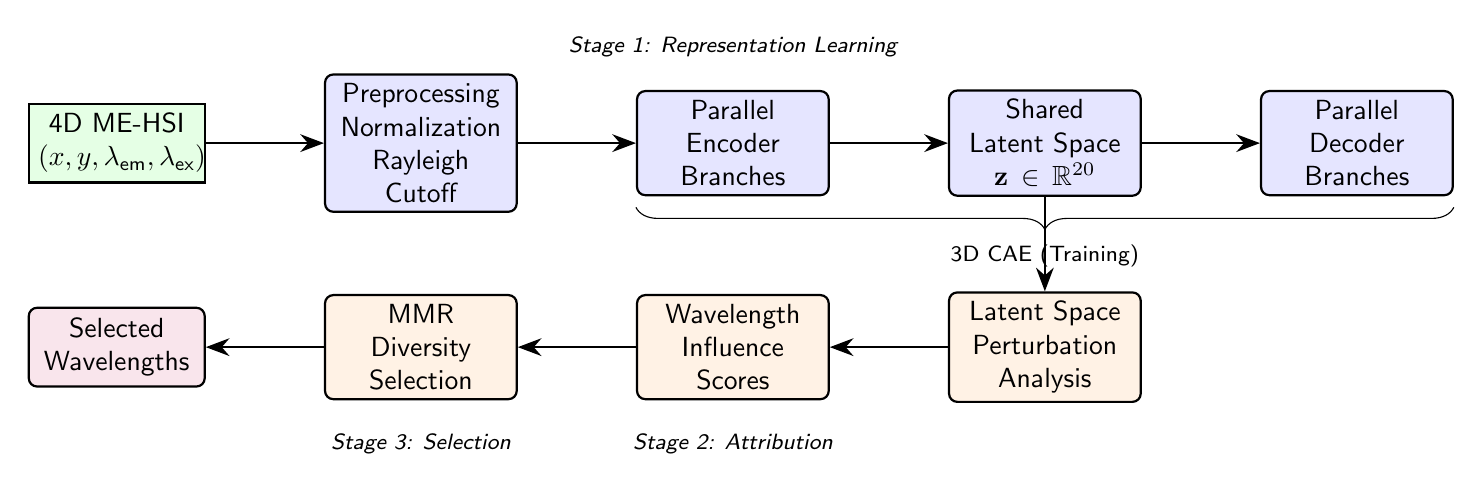
\begin{tikzpicture}[
    node distance=1.5cm,
    block/.style={rectangle, draw=black, thick, fill=blue!10, text width=2.2cm, minimum height=1.2cm, align=center, rounded corners=3pt},
    data/.style={rectangle, draw=black, thick, fill=green!10, text width=2cm, minimum height=1cm, align=center},
    process/.style={rectangle, draw=black, thick, fill=orange!10, text width=2.2cm, minimum height=1.2cm, align=center, rounded corners=3pt},
    output/.style={rectangle, draw=black, thick, fill=purple!10, text width=2cm, minimum height=1cm, align=center, rounded corners=3pt},
    arrow/.style={-{Stealth[length=3mm]}, thick}
]

\node[data] (input) {4D ME-HSI\\$(x,y,\lambdaem,\lambdaex)$};

\node[block, right=of input] (preprocess) {Preprocessing\\Normalization\\Rayleigh Cutoff};

\node[block, right=of preprocess] (encoder) {Parallel\\Encoder\\Branches};
\node[block, right=of encoder] (latent) {Shared\\Latent Space\\$\vect{z} \in \R^{20}$};
\node[block, right=of latent] (decoder) {Parallel\\Decoder\\Branches};

\node[process, below=1.2cm of latent] (perturb) {Latent Space\\Perturbation\\Analysis};

\node[process, left=of perturb] (influence) {Wavelength\\Influence\\Scores};

\node[process, left=of influence] (mmr) {MMR\\Diversity\\Selection};

\node[output, left=of mmr] (output) {Selected\\Wavelengths};

\draw[arrow] (input) -- (preprocess);
\draw[arrow] (preprocess) -- (encoder);
\draw[arrow] (encoder) -- (latent);
\draw[arrow] (latent) -- (decoder);
\draw[arrow] (latent) -- (perturb);
\draw[arrow] (perturb) -- (influence);
\draw[arrow] (influence) -- (mmr);
\draw[arrow] (mmr) -- (output);

\node[above=0.3cm of encoder, font=\footnotesize\itshape] {Stage 1: Representation Learning};
\node[below=0.3cm of influence, font=\footnotesize\itshape] {Stage 2: Attribution};
\node[below=0.3cm of mmr, font=\footnotesize\itshape] {Stage 3: Selection};

\draw[decorate, decoration={brace, amplitude=8pt, mirror, raise=4pt}]
    (encoder.south west) -- (decoder.south east) node[midway, below=14pt, font=\footnotesize] {3D CAE (Training)};

\end{tikzpicture}
\caption{Overview of the proposed wavelength selection framework. The pipeline comprises three stages: (1) a 3D CAE learns a compressed representation of 4D ME-HSI data; (2) perturbation analysis attributes latent dimensions to individual wavelengths; (3) MMR selection identifies diverse, informative band subsets.}
\label{fig:pipeline}
\end{figure*}

\subsection{Data Preprocessing}
\label{sec:preprocessing}

Raw ME-HSI acquisitions required several preprocessing steps before autoencoder training. (Figure~\ref{fig:pipeline})

\subsubsection{Intensity Normalization}
Fluorescence intensity depends on excitation source power and exposure time, which may vary across acquisitions.
Since the LED-based multi-excitation source operated at different power levels and exposure times for each excitation wavelength, raw intensities were normalized to ensure comparability across excitation channels:
\begin{equation}
I_{\text{norm}}(x, y, \lambdaem, \lambdaex) = \frac{I_{\text{raw}}(x, y, \lambdaem, \lambdaex)}{t_{\text{exp}}} \times \frac{t_{\text{ref}} \cdot P_{\text{ref}}}{P(\lambdaex)}
\label{eq:normalization}
\end{equation}
where $t_{\text{exp}}$ is the exposure time and $P(\lambdaex)$ is the lamp power at excitation wavelength $\lambdaex$.
The reference values $t_{\text{ref}}$ and $P_{\text{ref}}$ were set to the maximum exposure time and maximum lamp power, respectively, across all excitation wavelengths, ensuring that the normalization factor scales intensities upward for weaker or shorter-exposed channels.
Global min-max normalization was then applied to scale all values to $[0, 1]$.

\subsubsection{Rayleigh Scattering Removal}
Elastic scattering produces artifacts at two spectral locations.
First-order Rayleigh scattering occurs when emission wavelength approaches excitation wavelength ($\lambdaem \approx \lambdaex$), therefore, a spectral cutoff with offset $\Delta\lambda = 40$\, nm excluded emission bands where $\lambdaem < \lambdaex + \Delta\lambda$.
Second-order Rayleigh scattering produces artifacts near $\lambdaem \approx 2\lambdaex$, therefore emission bands within $\pm 40$\, nm of this harmonic were also excluded.
Together, these cutoffs resulted in variable numbers of valid emission bands per excitation, yielding 192 valid excitation-emission pairs from the original acquisition grid.

\subsubsection{Background Masking}
Non-sample regions (background) provide no discriminative information and may bias the autoencoder toward reconstructing uninformative patterns.
Binary masks $M(x, y) \in \{0, 1\}$ were generated through intensity thresholding or manual annotation, excluding background pixels from both training and evaluation.

\subsection{3D CAE}
\label{sec:architecture}

The central architectural challenge in processing 4D ME-HSI data was the variable spectral dimension across excitations.
After the Rayleigh cutoff, each excitation wavelength $\lambdaex$ yielded a different number of valid emission bands $N_{\text{em}}(\lambdaex)$.
A monolithic architecture would require padding and masking complexities to address the varying emission wavelength counts for each excitation; instead, a parallel-branch design was employed where each excitation is processed by a dedicated encoder branch, with features merged into a shared latent representation.

\subsubsection{Encoder Architecture}
For each excitation wavelength $\lambdaex^{(i)}$, $i = 1, \ldots, N_{\text{ex}}$, an encoder branch was defined, comprising a 3D convolutional layer that processes the spatial-spectral cube:
\begin{equation}
\vect{h}^{(i)} = \sigma\left(\text{Conv3D}\left(\vect{X}^{(i)}\right)\right)
\label{eq:encoder}
\end{equation}
where $\vect{X}^{(i)} \in \R^{H \times W \times N_{\text{em}}^{(i)}}$ is the input cube for excitation $i$, Conv3D applies $k_1 = 20$ filters of size $5 \times 5 \times \min(5, N_{\text{em}}^{(i)})$, and $\sigma$ is the sigmoid activation function.
The subscripts in $k_1$ and $k_3$ (introduced below) index the first and third convolutional layers; the intermediate feature-merging step has no learned parameters.
The adaptive spectral kernel size accommodated variable band counts across excitations.

After convolution, adaptive average pooling standardized the spectral dimension to 1, yielding feature maps $\vect{h}^{(i)} \in \R^{k_1 \times H \times W}$ with consistent dimensions across excitations.
Dropout regularization (rate 0.5) was applied after pooling to prevent overfitting.

\subsubsection{Feature Merging}
The excitation-specific feature maps were combined through element-wise averaging:
\begin{equation}
\bar{\vect{h}} = \frac{1}{N_{\text{ex}}} \sum_{i=1}^{N_{\text{ex}}} \vect{h}^{(i)}
\label{eq:merge}
\end{equation}
This merging strategy offers several advantages over alternatives.
Concatenation would yield feature dimensionality that grows with $N_{\text{ex}}$, increasing model complexity.
Averaging provided implicit noise reduction and was robust to intensity variations across excitations.
The merged features $\bar{\vect{h}}$ captured cross-excitation correlations by integrating patterns from all excitation branches.

\subsubsection{Shared Latent Space}
An additional convolutional layer transformed the merged features into the latent representation:
\begin{equation}
\vect{z} = \sigma\left(\text{Conv3D}\left(\bar{\vect{h}}\right)\right)
\label{eq:latent}
\end{equation}
where $\vect{z} \in \R^{k_3 \times 1 \times H \times W}$ with $k_3 = 20$ channels constitutes the bottleneck encoding.
This latent space $\vect{z}$ encapsulates the essential structure of the 4D ME-HSI data in a compressed form.
The perturbation analysis (Section~\ref{sec:perturbation}) probes this space to identify which wavelengths contribute most to the learned representation.

\subsubsection{Decoder Architecture}
The decoder mirrors the encoder with symmetric structure.
A shared decoding layer transformed the latent representation:
\begin{equation}
\vect{g} = \sigma\left(\text{Conv3D}\left(\vect{z}\right)\right)
\label{eq:decode_shared}
\end{equation}
yielding features $\vect{g} \in \R^{k_1 \times 1 \times H \times W}$.
Parallel decoder branches then reconstructed each excitation's spectral cube:
\begin{equation}
\hat{\vect{X}}^{(i)} = \sigma\left(\text{Conv3D}^{(i)}\left(\vect{g}\right)\right)
\label{eq:decode_branch}
\end{equation}
where $\text{Conv3D}^{(i)}$ maps from $k_1$ to $N_{\text{em}}^{(i)}$ channels.
Figure~\ref{fig:architecture} illustrates the complete architecture.

\begin{figure*}[!t]
\centering
\resizebox{\textwidth}{!}{%
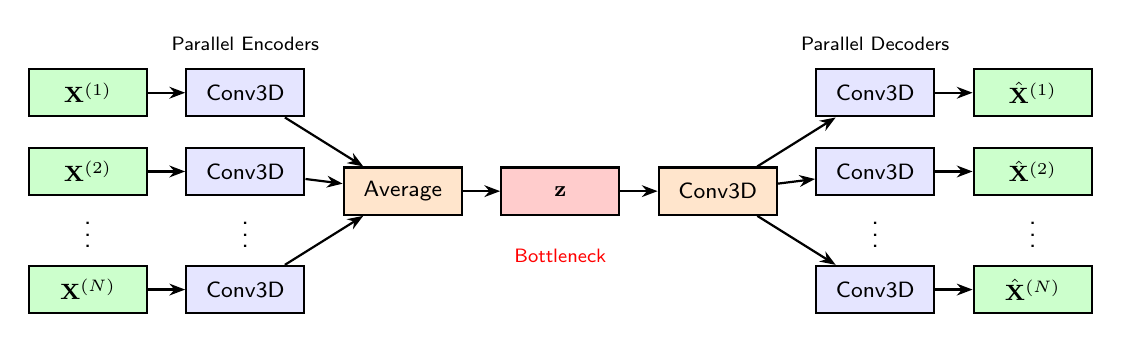
\begin{tikzpicture}[
    scale=1,
    transform shape,
    block/.style={rectangle, draw, thick, fill=blue!10, minimum width=1.5cm, minimum height=0.6cm, align=center, font=\footnotesize},
    arrow/.style={-{Stealth[length=2mm]}, thick},
    label/.style={font=\scriptsize}
]

% Input branches
\node[block, fill=green!20] at (0, 2) (in1) {$\vect{X}^{(1)}$};
\node[block, fill=green!20] at (0, 1) (in2) {$\vect{X}^{(2)}$};
\node at (0, 0.3) {$\vdots$};
\node[block, fill=green!20] at (0, -0.5) (inN) {$\vect{X}^{(N)}$};

% Encoder branches
\node[block] at (2, 2) (enc1) {Conv3D};
\node[block] at (2, 1) (enc2) {Conv3D};
\node at (2, 0.3) {$\vdots$};
\node[block] at (2, -0.5) (encN) {Conv3D};

% Merge
\node[block, fill=orange!20] at (4, 0.75) (merge) {Average};

% Latent
\node[block, fill=red!20] at (6, 0.75) (latent) {$\vect{z}$};

% Shared decode
\node[block, fill=orange!20] at (8, 0.75) (dec_shared) {Conv3D};

% Decoder branches
\node[block] at (10, 2) (dec1) {Conv3D};
\node[block] at (10, 1) (dec2) {Conv3D};
\node at (10, 0.3) {$\vdots$};
\node[block] at (10, -0.5) (decN) {Conv3D};

% Output branches
\node[block, fill=green!20] at (12, 2) (out1) {$\hat{\vect{X}}^{(1)}$};
\node[block, fill=green!20] at (12, 1) (out2) {$\hat{\vect{X}}^{(2)}$};
\node at (12, 0.3) {$\vdots$};
\node[block, fill=green!20] at (12, -0.5) (outN) {$\hat{\vect{X}}^{(N)}$};

% Arrows
\foreach \i in {1,2,N} {
    \draw[arrow] (in\i) -- (enc\i);
    \draw[arrow] (dec\i) -- (out\i);
}
\draw[arrow] (enc1) -- (merge);
\draw[arrow] (enc2) -- (merge);
\draw[arrow] (encN) -- (merge);
\draw[arrow] (merge) -- (latent);
\draw[arrow] (latent) -- (dec_shared);
\draw[arrow] (dec_shared) -- (dec1);
\draw[arrow] (dec_shared) -- (dec2);
\draw[arrow] (dec_shared) -- (decN);

% Labels
\node[above=0.1cm of enc1, label] {Parallel Encoders};
\node[above=0.1cm of dec1, label] {Parallel Decoders};
\node[below=0.3cm of latent, label, text=red] {Bottleneck};

\end{tikzpicture}%
}
\caption{3D CAE architecture with parallel branches. Each excitation is processed by a dedicated encoder branch; features are averaged into a shared latent space; parallel decoder branches reconstruct the original 4D structure.}
\label{fig:architecture}
\end{figure*}

\subsubsection{Loss Function and Training}
The autoencoder was trained to minimize masked mean squared error:
\begin{equation}
\mathcal{L} = \frac{1}{N_{\text{valid}}} \sum_{i=1}^{N_{\text{ex}}} \sum_{x,y} M(x,y) \cdot \left\| \vect{X}^{(i)}_{x,y} - \hat{\vect{X}}^{(i)}_{x,y} \right\|^2
\label{eq:loss}
\end{equation}
where $M(x,y)$ is the background mask, $N_{\text{valid}}$ is the number of valid pixels, and the sum runs over all excitations and spatial locations.
Masking ensured the network focused on sample regions rather than background.

Training employed the Adam optimizer~\cite{kingma2014adam} with learning rate $\eta = 0.001$, learning rate scheduling (ReduceOnPlateau with factor 0.5 and patience 5), and early stopping (patience 5 epochs).
Large images were partitioned into $64 \times 64$ patches with 8-pixel overlap for batch training; typical convergence occurred within 25--30 epochs.

\subsection{Perturbation-Based Wavelength Attribution}
\label{sec:perturbation}

The trained autoencoder learned a compressed representation that captures the essential structure of ME-HSI data.
Different latent dimensions encode different aspects of this structure; the goal was to attribute each latent dimension's influence back to specific excitation-emission wavelength pairs.
If perturbing a latent dimension significantly changed the reconstruction of a particular wavelength, that wavelength must be encoded by that dimension.
The rationale follows from the autoencoder objective: a latent space trained to reconstruct the full 4D cube must retain whatever information the reconstruction requires~\cite{hinton2006reducing}, so wavelengths that are redundant or dominated by noise contribute little to it.
Tracing which excitation-emission pairs respond most strongly when a latent dimension is displaced therefore reveals the wavelengths on which the learned representation depends; the perturbation mechanism below performs this tracing, and the MMR step (Section~\ref{sec:mmr}) then removes redundancy among the wavelengths it identifies.

\subsubsection{Latent Dimension Scoring}
Not all latent dimensions carry equal information.
The $k_3 = 20$ latent dimensions were first ranked by importance using variance-based scoring:
\begin{equation}
\text{score}(d) = \text{Var}_{\text{samples}}\left(\vect{z}[\cdot, d, \cdot, \cdot, \cdot]\right)
\label{eq:dim_score}
\end{equation}
where $\vect{z}[\cdot, d, \cdot, \cdot, \cdot]$ denotes dimension $d$ across all samples and spatial locations.
Higher variance indicated that the dimension captured meaningful variation rather than constant or near-zero values.
The top $k$ dimensions were then selected for perturbation analysis, where $k$ is treated as a hyperparameter; empirical evaluation (Section~\ref{sec:results}) revealed that PCA-based dimension selection (Section~\ref{sec:implementation}) with $k = 3$ achieved optimal performance.

Alternative scoring methods include activation magnitude (mean absolute value) and reconstruction sensitivity (MSE when dimension is zeroed).
PCA-based scoring yielded the most consistent wavelength rankings, likely because its leading components captured the primary modes of spectral variation that distinguish different materials.

\subsubsection{Systematic Perturbation}
For each selected latent dimension $d$, the perturbed representations were generated in both directions by one of two schemes, a percentile scheme and an absolute-range scheme:
\begin{align}
\vect{z}^{\pm}_d &= \vect{z} + \left( Q_{50 \pm \epsilon/2}(z_d) - \bar{z}_d \right) \vect{e}_d \label{eq:perturb_pos}\\
\vect{z}^{\pm}_d &= \vect{z} \pm \tfrac{\epsilon}{100} \left( \max z_d - \min z_d \right) \vect{e}_d \label{eq:perturb_neg}
\end{align}
where $\vect{e}_d$ is a one-hot vector selecting dimension $d$, $Q_p(z_d)$ (rounded to the nearest tabulated percentile) and $\bar{z}_d$ are the $p$-th percentile and the mean of dimension $d$ across the analysis samples, $\max z_d - \min z_d$ is its observed range, and $\epsilon$ controls perturbation magnitude.
Values of $\epsilon \in \{30, 40, 50\}$ (medium) and $\epsilon \in \{50, 60, 70\}$ (high) were used, and results across the three magnitudes were aggregated to ensure robustness.
Scaling the displacement to the empirical distribution of each dimension ensured perturbations proportional to its natural variation, avoiding both negligibly small and destructively large perturbations.

\subsubsection{Sensitivity Mapping}
Decoding the perturbed representations yielded reconstructions $\hat{\vect{X}}^{+}_d$ and $\hat{\vect{X}}^{-}_d$.
The sensitivity of each wavelength to perturbation in dimension $d$ was computed:
\begin{equation}
\begin{split}
\Delta_d(\lambdaex, \lambdaem) = \tfrac{1}{2}\Big( &\left| \hat{X}^{+}_d(\lambdaex, \lambdaem) - \hat{X}(\lambdaex, \lambdaem) \right| \\
&+ \left| \hat{X}^{-}_d(\lambdaex, \lambdaem) - \hat{X}(\lambdaex, \lambdaem) \right| \Big)
\end{split}
\label{eq:sensitivity}
\end{equation}
where $\hat{X}$ is the unperturbed reconstruction and averaging was performed over spatial locations and samples.
This quantifies how strongly each wavelength's reconstruction responds to displacements of latent dimension $d$.

\subsubsection{Influence Accumulation}
Sensitivity was accumulated across latent dimensions, weighted by dimension importance:
\begin{equation}
\text{Influence}(\lambdaex, \lambdaem) = \sum_{d \in \text{top-}k} \text{score}(d) \cdot \overline{\Delta_d(\lambdaex, \lambdaem)}
\label{eq:influence}
\end{equation}
where $\overline{\Delta_d}$ denotes the mean sensitivity across perturbation magnitudes.
The result is an influence matrix $\mat{I} \in \R^{N_{\text{ex}} \times \max(N_{\text{em}})}$ assigning importance scores to each excitation-emission pair.

\subsection{Maximum Marginal Relevance Selection}
\label{sec:mmr}

Selecting the top-$K$ wavelengths by influence score alone may yield redundant bands.
Adjacent wavelengths often captured correlated fluorescence patterns; a diverse selection covering different spectral regions may be more informative than a concentrated selection.
Maximum Marginal Relevance (MMR)~\cite{carbonell1998use} was adapted from information retrieval to balance relevance with diversity.

\subsubsection{MMR Formulation}
Given the set of all wavelength pairs $\mathcal{W}$ and a partial selection $\mathcal{S}$, MMR scores the next candidate as:
\begin{equation}
\text{MMR}(w_i) = \lambda \cdot \text{Rel}(w_i) - (1 - \lambda) \cdot \max_{w_j \in \mathcal{S}} \text{Sim}(w_i, w_j)
\label{eq:mmr}
\end{equation}
where $\text{Rel}(w_i)$ is the normalized influence score, $\text{Sim}(w_i, w_j)$ is the cosine similarity between spectral profiles at wavelengths $w_i$ and $w_j$, and $\lambda \in [0, 1]$ controls the relevance-diversity trade-off.

At $\lambda = 1$, MMR reduces to pure relevance ranking; at $\lambda = 0$, selection maximizes diversity without regard for informativeness.
The value $\lambda = 0.5$ was fixed a priori, giving equal weight to both criteria~\cite{carbonell1998use}.

\subsubsection{Selection Procedure}
Algorithm~\ref{alg:mmr} presents the greedy MMR selection procedure.
The algorithm iteratively selected the wavelength that maximized the MMR score until $K$ wavelengths were chosen.
The output is an ordered list of excitation-emission pairs, ranked by selection order, enabling flexible thresholding based on accuracy-efficiency trade-offs.

\begin{algorithm}[t]
\caption{MMR Wavelength Selection}
\label{alg:mmr}
\begin{algorithmic}[1]
\REQUIRE Wavelength set $\mathcal{W}$, influence matrix $\mat{I}$, target count $K$, trade-off parameter $\lambda$
\ENSURE Selected wavelength set $\mathcal{S}$
\STATE Initialize $\mathcal{S} \gets \emptyset$
\STATE Compute $\text{Rel}(w) \gets \mat{I}(w) / \max(\mat{I})$ for all $w \in \mathcal{W}$
\FOR{$i = 1$ to $K$}
    \FOR{each $w \in \mathcal{W} \setminus \mathcal{S}$}
        \IF{$\mathcal{S} = \emptyset$}
            \STATE $\text{MMR}(w) \gets \text{Rel}(w)$
        \ELSE
            \STATE $\text{MMR}(w) \gets \lambda \cdot \text{Rel}(w) - (1-\lambda) \cdot \max_{w_j \in \mathcal{S}} \text{Sim}(w, w_j)$
        \ENDIF
    \ENDFOR
    \STATE $w^* \gets \arg\max_{w \in \mathcal{W} \setminus \mathcal{S}} \text{MMR}(w)$
    \STATE $\mathcal{S} \gets \mathcal{S} \cup \{w^*\}$
\ENDFOR
\RETURN $\mathcal{S}$
\end{algorithmic}
\end{algorithm}

\subsection{Validation Protocol}
\label{sec:validation}

The wavelength selection pipeline (Sections~\ref{sec:architecture}--\ref{sec:mmr}) is entirely unsupervised and operates without access to class labels.
A supervised classification algorithm is used to quantify how much discriminative power remains in the compressed features; the classification described below serves \emph{only} to evaluate the quality of selected wavelengths---it does not influence the selection process.
The labels play the same validating role in choosing among the attribution configurations of Section~\ref{sec:configurations}: every configuration produces its wavelength ranking without labels, and the classifier is then used to determine which configuration yielded the most informative selection.
In a deployment scenario, wavelength selection would proceed identically whether or not labeled data exists.

For each pixel $(x, y)$ with ground-truth labels, spectral values at the $K$ selected wavelength pairs form the feature vector:
\begin{equation}
\resizebox{0.88\columnwidth}{!}{$
\vect{f}(x, y) = \left[ I(x, y, \lambda_{\mathrm{em}}^{(1)}, \lambda_{\mathrm{ex}}^{(1)}), \ldots, I(x, y, \lambda_{\mathrm{em}}^{(K)}, \lambda_{\mathrm{ex}}^{(K)}) \right]^\top$},
\label{eq:features}
\end{equation}
where $(\lambdaem^{(k)}, \lambdaex^{(k)})$ is the $k$-th selected pair.
Features were standardized (zero mean, unit variance) and classified using a $k$-nearest neighbors (KNN) classifier~\cite{cover1967nearest} with 5 neighbors and Euclidean distance.
This non-parametric classifier was chosen to isolate the effect of wavelength selection from classifier capacity.
A baseline using all 192 bands with the same classifier established the performance reference.
Cohen's Kappa ($\kappa$)~\cite{cohen1960coefficient}, classification accuracy, and weighted F1-score served as primary evaluation metrics; the complete metric set is defined in Section~\ref{sec:metrics}.
\section{Experimental Setup}
\label{sec:experimental_setup}
\subsection{Datasets}
\label{sec:datasets}

Two fluorescence datasets were used. The lichen dataset served as the primary benchmark for the full configuration sweep and robustness analysis; the collagen sponge dataset provided an independent test of cross-domain generalization.

\subsubsection{Lichen Dataset}
\label{sec:dataset_lichen}

The primary dataset comprised ME-HSI acquisitions of lichen specimens---composite organisms formed by symbiotic associations between fungi and photosynthetic partners (algae or cyanobacteria).
The lichen species used in this study are shown in Figure~\ref{fig:lichen_rgb}.
Lichens serve as important bioindicators for environmental monitoring, and their autofluorescence signatures reflect both fungal and algal components~\cite{meysurova2021optical}.\\
\textbf{Lichen Specimen Collection and Identification:} Wild specimens of Ramalina sinensis, Ramalina fraxinea, and Flavopunctelia soredica were collected from Tavush Province of Armenia in the Fall of 2023-24. Sample collection was conducted in accordance with relevant national and institutional guidelines. Taxonomic identification of the wild lichen specimens was confirmed by expert lichenologist Dr. Arsen Garparyan. Voucher specimens have been deposited in the Herbarium of the Institute of Botany after A. Takhtajyan (ERE) with the following accession numbers: Ramalina sinensis (LICH-840), Ramalina fraxinea (LICH-841), and Flavopunctelia soredica (LICH-842).

\begin{table}[!t]
\centering
\caption{Lichen Dataset Specifications}
\label{tab:dataset}
\begin{tabular}{@{}ll@{}}
\toprule
\textbf{Parameter} & \textbf{Value} \\
\midrule
Spatial dimensions & $1040 \times 925$ pixels \\
Excitation wavelengths & 8 (310, 325, 340, 365, 385, 400, 415, 430\,nm) \\
Emission range & 420--720\,nm \\
Emission bands (per ex.) & 22--28 (variable after Rayleigh cutoff) \\
Total EEM pairs & 192 \\
Spectral resolution & $\sim$12.5\,nm \\
Ground-truth classes & 4 distinct classes \\
\bottomrule
\end{tabular}
\end{table}

Table~\ref{tab:dataset} summarizes the dataset details.
The acquisition system employed an LED-based multi-excitation source (WheeLED, Mightex, Toronto, CA) spanning the 310 - 440\,nm range. Images were acquired with a Nuance FX hyperspectral camera (PerkinElmer, Waltham, MA), capturing emission spectra from 420 to 720\,nm with 10\,nm step at each excitation.
Exposure times and LED power were recorded for intensity normalization per Equation~\eqref{eq:normalization}.

Ground-truth annotations were generated based on the knowledge of the origins of each lichen species obtained from the Takhtajyan Institute of Botany, National Academy of Sciences of Armenia~\cite{chilingaryan2025whispers}.
Four regions were delineated, providing ground-truth annotations for supervised evaluation.
The total of 192 valid excitation-emission pairs results from variable emission windows after first- and second-order Rayleigh scattering removal (Section~\ref{sec:preprocessing}).

\begin{figure}[!t]
\centering
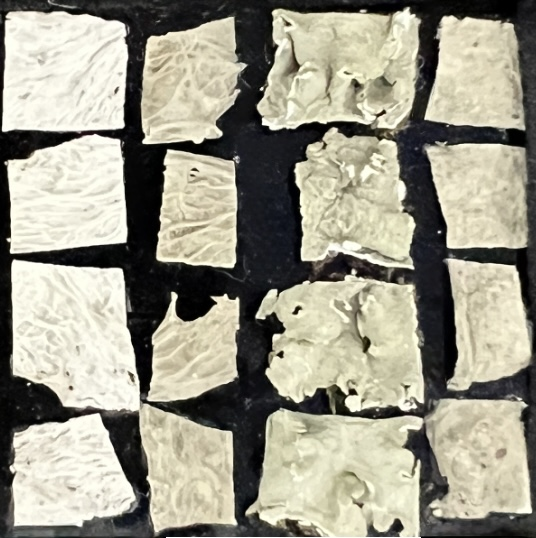
\includegraphics[width=0.45\textwidth]{figures/LichensRGB.jpg}
\caption{Visual appearance of lichens used in this study. The first two columns are ~7x7 mm pieces of Ramalina Sinesis (back and front). The third and fourth columns are Flavopunctelia Soredica and Ramalina Fraxinea, respectively (both front surfaces). }
\label{fig:lichen_rgb}
\end{figure}

\begin{figure}[!t]
\centering
\includegraphics[width=0.48\textwidth]{figures/LichensLabels_and_ROI.png}
\caption{Ground-truth annotation and baseline classification results using all 192 bands. The 16 lichen specimens are arranged in a $4 \times 4$ grid, with columns corresponding to the four classes. Equal-sized square ROIs (one per class, $50 \times 60$ pixels each) in the first row provide training exemplars for KNN evaluation. These ROIs were used \emph{only} for post-hoc validation of wavelength selection quality; they did not influence the unsupervised selection pipeline.}
\label{fig:roi_overlay}
\end{figure}

\subsubsection{Collagen Sponge Dataset}
\label{sec:dataset_collagen}

A second dataset comprised ME-HSI acquisitions of collagen sponge specimens. Collagen sponges were fabricated from purified Type~I collagen derived from bovine tendon followed by chemical crosslinking with glutaraldehyde at three different concentrations (0.002, 0.0075, and 0.013\%).
\\
\textbf{Tissue Sourcing and Collagen Extraction:} Type I collagen was extracted from bovine trotters obtained post-mortem from a local licensed abattoir. Tissues were collected as animal by-products from routine commercial food production.
\\
Collagen autofluorescence in the near-UV and blue range is an established structural biomarker, and the crosslinker concentration modulates the supramolecular organization of collagen fibrils, producing measurable shifts in both emission peak position and intensity~\cite{lakowicz2006principles}.

This dataset evaluates whether the framework, developed on lichen biology, transfers to a chemically distinct fluorophore family without modification.

\begin{table}[!t]
\centering
\caption{Collagen Sponge Dataset Specifications}
\label{tab:dataset_collagen}
\begin{tabular}{@{}ll@{}}
\toprule
\textbf{Parameter} & \textbf{Value} \\
\midrule
Excitation wavelengths & 6 (310, 325, 340, 365, 385, 400\,nm) \\
Emission range & 420--720\,nm \\
Total EEM pairs & 158 \\
Spectral resolution & 10\,nm \\
Ground-truth classes & 3 crosslinker concentrations \\
Annotated pixels & 39{,}970 \\
\bottomrule
\end{tabular}
\end{table}

Table~\ref{tab:dataset_collagen} summarizes the collagen sponge dataset specifications.
The same camera and emission grid were used as for the lichen dataset, with six excitation wavelengths from 310 to 400\,nm. After first- and second-order Rayleigh scattering removal, 158 valid excitation-emission pairs remained, a different spectral coverage from the lichen benchmark, so the wavelength selection task is genuinely new rather than a repetition on the same grid.
Ground-truth annotations were generated by manual labeling of nine sponge specimens arranged in a $3 \times 3$ grid, with columns corresponding to the three crosslinker-concentration classes (Figure~\ref{fig:collagen_roi}).
For each class, a small interior square ROI in one specimen of the first row provides the labeled training pixels for the downstream classifier; the remaining annotated pixels form the evaluation set.
As with the lichen dataset, these ROIs were used \emph{only} for post-hoc validation and did not influence the unsupervised selection pipeline.

\begin{figure}[!t]
\centering
\includegraphics[width=0.46\textwidth]{figures/collagen_roi.png}
\caption{Ground-truth annotation and class layout for the collagen sponge dataset. Nine specimens are arranged in a $3 \times 3$ grid, with columns corresponding to the three crosslinker-concentration classes. The white interior squares (top row) mark the small ROIs used as supervised training exemplars; the remainder of each specimen forms the evaluation set.}
\label{fig:collagen_roi}
\end{figure}

\subsection{Implementation Details}
\label{sec:implementation}

The framework was implemented in Python 3.10 using PyTorch 2.0~\cite{paszke2019pytorch} for deep learning components and scikit-learn 1.3~\cite{pedregosa2011scikit} for classification and metrics.
All experiments were conducted on a workstation with an NVIDIA RTX 4070 GPU (8\,GB VRAM) and 64\,GB system RAM.

\subsubsection{Autoencoder Hyperparameters}
Table~\ref{tab:hyperparams} lists the autoencoder configuration.
$k_1 = k_3 = 20$ filters were employed based on preliminary experiments showing this provided sufficient capacity without overfitting.
The $5 \times 5$ spatial filter captured local texture patterns relevant for biological specimens.
Sigmoid activations ensured outputs remained in $[0, 1]$, matching the normalized input range.

\begin{table}[!t]
\centering
\caption{Autoencoder Hyperparameters}
\label{tab:hyperparams}
\begin{tabular}{@{}lll@{}}
\toprule
\textbf{Parameter} & \textbf{Value} & \textbf{Rationale} \\
\midrule
Encoder filters ($k_1$) & 20 & Capacity vs.~complexity \\
Latent filters ($k_3$) & 20 & Bottleneck dimensionality \\
Spatial filter size & $5 \times 5$ & Local pattern capture \\
Spectral filter size & min(5, $N_{\text{em}}$) & Variable band counts \\
Activation & Sigmoid & Match $[0,1]$ input \\
Dropout rate & 0.5 & Regularization \\
Patch size & $64 \times 64$ & GPU memory constraints \\
Patch overlap & 8 pixels & Boundary continuity \\
Batch size & 32 & Training stability \\
Optimizer & Adam~\cite{kingma2014adam} & Adaptive learning rates \\
Initial learning rate & 0.001 & Standard default \\
LR scheduler & ReduceOnPlateau & Convergence refinement \\
LR factor & 0.5 & Reduction magnitude \\
Patience (LR) & 5 epochs & Schedule sensitivity \\
Early stopping patience & 5 epochs & Prevent overfitting \\
\bottomrule
\end{tabular}
\end{table}

\subsubsection{Perturbation Analysis Parameters}
For latent space analysis, dimensions were ranked by either variance (as in Section~\ref{sec:perturbation}) or by their contribution to a Principal Component Analysis (PCA) decomposition of the latent space.
Both methods were explored at $k \in \{1, 3\}$ top dimensions. Perturbations were applied using two methods, percentile-based and absolute-range (Section~\ref{sec:perturbation}), at medium ($\epsilon \in \{30, 40, 50\}$) and high ($\epsilon \in \{50, 60, 70\}$) magnitude levels.
The best configurations of Table~\ref{tab:main_results} were obtained with the percentile scheme and the medium magnitude set, except the 30- and 9-band rows (absolute range, medium) and the 50-band row (percentile, high).
Sensitivity values were averaged across 1,000 randomly sampled patches to ensure robust estimation.
Additionally, three normalization strategies for influence scores were compared: no normalization, max-per-excitation, and variance normalization (see Section~\ref{sec:results}).

\subsubsection{MMR Configuration}
The MMR selection used $\lambda = 0.5$ (equal weight to relevance and diversity), with spectral similarity computed as cosine similarity between full spectral profiles at each wavelength pair.

\subsubsection{Classification Setup}
KNN classification employed 5 neighbors with Euclidean distance metric.
Features were standardized using z-score normalization (zero mean, unit variance).
For evaluation, all annotated pixels were used, with four regions of interest (ROIs) providing class exemplars (Figure~\ref{fig:roi_overlay}); the same classifier configuration was applied consistently across all experiments for fair comparison.

\subsection{Experimental Configurations}
\label{sec:configurations}

Multiple configurations were evaluated, varying the parameters of each framework component.
Table~\ref{tab:configs} summarizes the configuration space explored.

\begin{table}[!t]
\centering
\caption{Configuration Parameter Space}
\label{tab:configs}
\begin{tabular}{@{}ll@{}}
\toprule
\textbf{Parameter} & \textbf{Values Tested} \\
\midrule
Dimension selection method & Variance, PCA \\
Number of dimensions ($k$) & 1, 3 \\
Perturbation method & Percentile, Absolute range \\
Perturbation magnitudes ($\epsilon$) & Medium \{30,40,50\}, High \{50,60,70\} \\
Normalization method & None, Max-per-excitation, Variance \\
MMR trade-off ($\lambda$) & 0.5 (fixed) \\
Number of bands selected & 1--180 (64 values) \\
\bottomrule
\end{tabular}
\end{table}

From the full configuration space, a comprehensive sweep of 3,072 experiments was conducted spanning all parameter combinations:
\begin{itemize}
    \item \textbf{Band count sweep:} 64 values from 1 to 180 bands (step 1 for 1--20, step 2 for 22--60, step 5 for 65--180). The upper bound of 180 was chosen because the full 192-band baseline is evaluated separately; near-baseline selections yield diminishing analytical value.
    \item \textbf{Attribution parameters:} Two dimension selection methods $\times$ two dimension counts $\times$ two perturbation methods $\times$ two magnitude levels $= 16$ configurations.
    \item \textbf{Normalization:} Three post-attribution normalization strategies to assess sensitivity to score scaling.
\end{itemize}
This yields $16 \times 3 = 48$ attribution--normalization configurations per band count, and $48 \times 64 = 3{,}072$ total experiments.

Each configuration produced a wavelength ranking through the unsupervised pipeline; classification accuracy was measured post-hoc to assess quality.

\subsection{Evaluation Metrics}
\label{sec:metrics}

Wavelength selection was evaluated through three groups of metrics.
\emph{Classification metrics} include accuracy, balanced accuracy, weighted precision/recall/F1-score, Cohen's Kappa ($\kappa$), and Matthews Correlation Coefficient (MCC).
\emph{Reconstruction metrics} include RMSE and PSNR (dB) between autoencoder input and output.
\emph{Reduction metrics} include data reduction ($1 - K/N_{\text{total}}$, where $K$ is the number of selected bands and $N_{\text{total}} = 192$) and relative performance (selected accuracy divided by the 192-band baseline accuracy).
All classification metrics were computed against the same KNN baseline using all 192 bands, providing a consistent reference for evaluating selection effectiveness.
\section{Results}
\label{sec:results}
\subsection{Autoencoder Performance}
\label{sec:results_autoencoder}

The 3D CAE converged reliably across multiple training runs, demonstrating stable representation learning for 4D ME-HSI data.

\subsubsection{Training Convergence}
Figure~\ref{fig:training} shows representative training curves.
The masked MSE loss decreased from approximately 0.45 to 0.03 over 25--30 epochs, with smooth convergence and no evidence of overfitting (training and validation losses tracked closely).
Learning rate reductions triggered at epochs 15 and 22 refined convergence.
Early stopping typically activated between epochs 25--30.

\begin{figure}[!t]
\centering
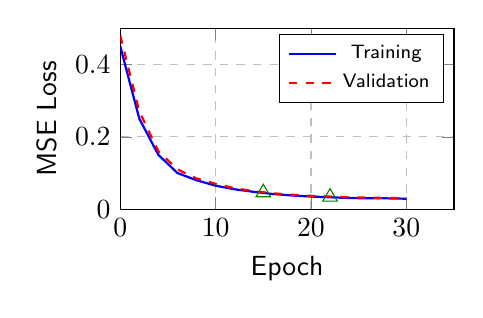
\begin{tikzpicture}
\begin{axis}[
    width=0.48\textwidth,
    height=0.32\textwidth,
    xlabel={Epoch},
    ylabel={MSE Loss},
    xmin=0, xmax=35,
    ymin=0, ymax=0.5,
    grid=major,
    grid style={dashed, gray!50},
    legend pos=north east,
    legend style={font=\scriptsize},
]

% Training loss curve
\addplot[blue, thick] coordinates {
    (0, 0.45) (2, 0.25) (4, 0.15) (6, 0.10) (8, 0.08) (10, 0.065)
    (12, 0.055) (14, 0.048) (16, 0.042) (18, 0.038) (20, 0.035)
    (22, 0.033) (24, 0.031) (26, 0.030) (28, 0.030) (30, 0.029)
};
\addlegendentry{Training}

% Validation loss curve
\addplot[red, thick, dashed] coordinates {
    (0, 0.48) (2, 0.27) (4, 0.16) (6, 0.11) (8, 0.085) (10, 0.070)
    (12, 0.058) (14, 0.050) (16, 0.044) (18, 0.040) (20, 0.037)
    (22, 0.035) (24, 0.033) (26, 0.032) (28, 0.031) (30, 0.031)
};
\addlegendentry{Validation}

% LR reduction markers
\addplot[only marks, mark=triangle, mark size=3pt, green!50!black] coordinates {(15, 0.046) (22, 0.034)};

\end{axis}
\end{tikzpicture}
\caption{Training convergence curves for the 3D CAE. Loss decreased smoothly from 0.45 to 0.03 over 30 epochs. Green triangles indicate learning rate reductions.}
\label{fig:training}
\end{figure}

\subsubsection{Reconstruction Quality}
The trained autoencoder achieved RMSE of 0.078 and PSNR of 22.16\,dB on the validation set.
Visual inspection confirmed that reconstructions preserved key spectral features across all excitation wavelengths.
Per-excitation analysis showed consistent reconstruction quality, with no systematic degradation at particular excitation wavelengths.

\subsubsection{Latent Space Quality}
Analysis of the 20-dimensional latent space revealed meaningful variation.
The top 5 dimensions by variance accounted for 72\% of total latent variance, indicating that information was distributed but concentrated in a subset of dimensions.
This supported using top-$k$ dimension selection for perturbation analysis.

\subsection{Wavelength Selection Results}
\label{sec:results_selection}

Using all 192 wavelength pairs with KNN classification established a baseline of 88.2\% accuracy ($\kappa = 0.842$).
Per-class performance varied: Class~1 achieved 99.1\% recall and 98.0\% precision, while Classes~2 and~3 showed mutual confusion (15,846 Class~3 pixels misclassified as Class~2), reflecting spectral overlap in their fluorescence signatures.
This confusion pattern persisted across all wavelength selections, indicating a fundamental limitation of the spectral data rather than the selection method.

Wavelength selection was evaluated across 3,072 configurations spanning the full parameter space (Table~\ref{tab:configs}).
Table~\ref{tab:main_results} presents the best-performing configurations at key band counts, all of which used PCA-based dimension selection (see Section~\ref{sec:results_params} for method comparison).

\begin{table*}[!t]
\centering
\caption{Wavelength Selection Performance Across Band Counts (Best Configuration per Band Count)}
\label{tab:main_results}
\begin{tabular}{@{}lcccccc@{}}
\toprule
\textbf{Configuration} & \textbf{Bands} & \textbf{Reduction} & \textbf{Accuracy} & \textbf{F1 (wtd)} & \textbf{$\kappa$} & \textbf{Rel.\ Perf.} \\
\midrule
Baseline (all 192 bands) & 192 & 0.0\% & 0.882 & 0.882 & 0.842 & 100.0\% \\
\midrule
\textbf{PCA, 3-dim, 80 bands} & \textbf{80} & \textbf{58.3\%} & \textbf{0.952} & \textbf{0.952} & \textbf{0.936} & \textbf{108.0\%} \\
PCA, 1-dim, 60 bands & 60 & 68.8\% & 0.945 & 0.945 & 0.926 & 107.2\% \\
PCA, 3-dim, 50 bands & 50 & 74.0\% & 0.940 & 0.941 & 0.920 & 106.7\% \\
PCA, 1-dim, 40 bands & 40 & 79.2\% & 0.932 & 0.932 & 0.908 & 105.7\% \\
PCA, 1-dim, 30 bands & 30 & 84.4\% & 0.930 & 0.931 & 0.906 & 105.5\% \\
PCA, 1-dim, 20 bands & 20 & 89.6\% & 0.917 & 0.918 & 0.889 & 104.0\% \\
PCA, 3-dim, 13 bands & 13 & 93.2\% & 0.902 & 0.902 & 0.868 & 102.3\% \\
PCA, 3-dim, 10 bands & 10 & 94.8\% & 0.897 & 0.898 & 0.863 & 101.8\% \\
\textbf{PCA, 3-dim, 9 bands} & \textbf{9} & \textbf{95.3\%} & \textbf{0.894} & \textbf{0.895} & \textbf{0.859} & \textbf{101.5\%} \\
PCA, 1-dim, 5 bands & 5 & 97.4\% & 0.870 & 0.871 & 0.826 & 98.7\% \\
PCA, 1-dim, 3 bands & 3 & 98.4\% & 0.827 & 0.827 & 0.768 & 93.8\% \\
\bottomrule
\vspace{0.2em}
\end{tabular}
\parbox{\textwidth}{\small\textit{Note:} Best configuration at each band count shown; all use PCA-based dimension selection with MMR $\lambda = 0.5$. Bold rows indicate key operating points. Rel.\ Perf.\ = accuracy/baseline accuracy. The ``dim'' attribute indicates the number of latent dimensions used ($k$); remaining parameters (perturbation method, magnitude, normalization) varied per row. Normalization combinations were evaluated at each band count.}
\end{table*}

\subsubsection{Key Finding: Performance Exceeds Baseline}
An important finding was that the selected subsets \emph{exceeded}
baseline performance. With 80 bands (58.3\% data reduction), the method achieved
\emph{95.2\% accuracy}, 7.1\% points above the 88.2\% baseline.
Even with only 9 bands, accuracy remained at 89.4\%, still exceeding the baseline.
This demonstrates that the full spectrum contains redundant or noisy bands that
hinder classification, and that peak performance occurs at an intermediate
selection level.
Performance remained above 90\% across a wide range (13--100 bands), indicating robust selection; even the minimal 3-band configuration achieved 82.7\% significantly above the random chance (25\%). Figure~\ref{fig:accuracy_vs_bands} visualizes the accuracy-reduction trade-off across all 3,072 configurations.

\begin{figure}[!t]
\centering
\includegraphics[width=0.48\textwidth]{figures/accuracy_envelope.png}
\caption{Classification accuracy envelope as a function of band count.}
\label{fig:accuracy_vs_bands}
\end{figure}

\subsubsection{Visual Classification Results}
Figure~\ref{fig:classification_visual} presents spatial classification maps for the baseline, 80-band, and 9-band configurations.
The 80-band selection (b) shows improved spatial homogeneity compared to the baseline (a), with reduced Class~2/Class~3 confusion and sharper specimen boundaries.
The 9-band selection (c) remains visually comparable to the baseline despite 95.3\% data reduction.
Residual confusion between Class~2 and Class~3 persists across all configurations, reflecting genuine spectral overlap between these Foliose morphological types rather than selection failure.

\begin{figure*}[!t]
\centering
\begin{tabular}{@{}c@{\hspace{4pt}}c@{\hspace{4pt}}c@{}}
\includegraphics[width=0.32\textwidth]{figures/Baseline.png} &
\includegraphics[width=0.32\textwidth]{figures/80bands-best.png} &
\includegraphics[width=0.32\textwidth]{figures/9bands-efficient.png} \\[2pt]
(a) Baseline: 192 bands & (b) 80 bands (58\% reduction) & (c) 9 bands (95\% reduction) \\
88.2\% accuracy & 95.2\% accuracy & 89.4\% accuracy \\
\end{tabular}
\caption{Spatial classification maps. The 16 specimens are arranged as shown in Figure~\ref{fig:lichen_rgb} }
\label{fig:classification_visual}
\end{figure*}


\subsection{Robustness Validation}
\label{sec:results_robustness}

To verify that the method's performance reflected genuine wavelength selectivity rather than chance, a robustness analysis was conducted.

\subsubsection{Random Selection Comparison}
The 13-band selection was compared against 10,000 randomly generated 13-band combinations from the 192 available wavelengths.
Table~\ref{tab:robustness} and Figure~\ref{fig:robustness_hist} demonstrate the clear advantage of the learned selection.

\begin{table}[!t]
\centering
\caption{Robustness Analysis: Learned vs.\ Random Selection (13 Bands)}
\label{tab:robustness}
\begin{tabular}{@{}lc@{}}
\toprule
\textbf{Metric} & \textbf{Value} \\
\midrule
\textbf{Learned Selection} & \textbf{0.9016} \\
\midrule
Random Mean & 0.4606 \\
Random Std & 0.0358 \\
Random Minimum & 0.3797 \\
Random Maximum & 0.5792 \\
Random Median & 0.4494 \\
\midrule
Learned vs.\ Random & \textbf{Outperformed all 10,000} \\
\bottomrule
\end{tabular}
\end{table}

\begin{figure}[!t]
\centering
\includegraphics[width=0.48\textwidth]{figures/robustness_histogram.png}
\caption{Distribution of classification accuracies for 10,000 randomly sampled 13-band combinations. The histogram shows that random selections cluster around 46\% accuracy (dashed lines indicate mean and median), while the learned selection (solid purple line at 90.2\%) lies far in the upper tail, outperforming every random combination tested.}
\label{fig:robustness_hist}
\end{figure}
\begin{itemize}
    \item The method achieved 90.2\% accuracy compared to a random mean of 46.1\%.
    \item The best random selection (57.9\%) fell 32\% points below the learned result.
    \item The CAE perturbation-based selection \emph{surpassed every random combination}: it outperformed all 10,000 random samples tested.
\end{itemize}

This validated that the perturbation-based attribution successfully identified informative wavelengths rather than benefiting from the random combinations.

\subsubsection{Statistical Significance}
The learned selection accuracy (0.902) lay 12 standard deviations above the random mean:
\begin{equation}
z = \frac{0.9016 - 0.4606}{0.0358} = 12.3\sigma
\end{equation}
This indicated high statistical significance ($p \ll 10^{-20}$).

\subsection{Object-Level Analysis}
\label{sec:results_objects}

Object-level analysis was conducted across 16 individual lichen specimens to understand how wavelength selection affected different samples (Table ~\ref{tab:objects}). 
The data shows that difficult-to-classify objects showed the most improvement:
\begin{itemize}
    \item \textbf{Object 12} (Class 3, lowest baseline): Accuracy improved from 40.9\% to 86.0\% (+110.3\% relative improvement).
    \item \textbf{Object 11} (Class 3): Improved from 58.5\% to 91.7\% (+56.8\% relative improvement).
    \item \textbf{Object 8} (Class 2): Improved from 72.8\% to 68.9\%---the only object showing slight decline, reflecting the persistent Class 2/3 spectral overlap.
    \item \textbf{Object 7} (Class 2): Improved from 74.0\% to 88.0\% (+18.9\% relative improvement).
\end{itemize}

This pattern suggested that the full 192-band spectrum contained wavelengths that were \emph{detrimental} to the classification of certain specimens, likely due to noise or interference patterns specific to their spectral signatures.
Wavelength selection removed these harmful bands, with 15 of 16 specimens showing improvement, and performance standard deviation decreasing from 0.172 to 0.079.


\begin{table}[!t]
\centering
\caption{Object-Level Performance Summary}
\label{tab:objects}
\begin{tabular}{@{}lcc@{}}
\toprule
\textbf{Statistic} & \textbf{Baseline} & \textbf{Best Selection} \\
\midrule
Mean Accuracy & 0.886 & 0.947 \\
Std Deviation & 0.172 & 0.079 \\
Minimum & 0.409 (Obj.\ 12) & 0.689 (Obj.\ 8) \\
Maximum & 0.998 (Obj.\ 4) & 1.000 (Obj.\ 1) \\
\midrule
Objects Improved & -- & 15/16 (94\%) \\
Objects Maintained & -- & 0/16 (0\%) \\
Objects Declined & -- & 1/16 (6\%) \\
\bottomrule
\end{tabular}
\end{table}


\subsection{Sensitivity Analysis}
\label{sec:results_params}


PCA-based latent dimension selection outperformed variance-based selection (95.2\% vs.\ 87.0\% best accuracy).
This finding demonstrated that PCA decomposition of the learned latent space more effectively identified the dimensions encoding discriminative information.
Notably, PCA achieved its peak accuracy at 80 bands, while variance-based selection required 175 bands to reach its (lower) peak, suggesting that PCA selects more informative wavelengths early in the ranking.
The variance-based method did not exceed the 88.2\% baseline at any band count, while every PCA configuration from 9 bands upward surpassed it.
The MMR parameter $\lambda$ was fixed at 0.5 throughout the sweep (Section~\ref{sec:configurations}).
The effectiveness of this relevance-diversity balance is demonstrated in the wavelength analysis below.

\subsection{Selected Wavelength Analysis}
\label{sec:results_wavelengths}

Figure~\ref{fig:wavelength_heatmap} presents a heatmap of mean wavelength importance across the 16 above-baseline configuration groups.
For each group, the complete wavelength ranking from the maximum-band experiment was used, and a normalized importance score was computed as $1 - (\text{rank} - 1) / \text{max\_rank}$, then averaged across groups. The 9-band configuration of Table~\ref{tab:main_results} comprises the following excitation/emission pairs (nm), in selection order: 310/520, 385/500, 325/570, 430/610, 400/510, 340/500, 365/520, 415/615 and 430/680, i.e., one band from each of the seven excitation sources between 310 and 415\,nm and two bands from the 430\,nm source, with emission bands spanning 500--680\,nm.
This near one-per-excitation pattern reflects the per-excitation normalization of this configuration, which ranks the strongest band of every excitation first.

\begin{figure*}[!t]
\centering
\includegraphics[width=\textwidth]{figures/wavelength_heatmap.png}
\caption{Mean wavelength importance score for the lichen dataset, across the 16 above-baseline configuration groups. Each cell shows the average normalized rank (1.0 = consistently top-ranked, 0.0 = lowest-ranked) for each excitation-emission pair. Grey cells indicate wavelengths excluded by Rayleigh scattering cutoffs.}
\label{fig:wavelength_heatmap}
\end{figure*}

\subsection{Cross-Dataset Validation: Collagen Sponges}
\label{sec:results_collagen}

To assess whether the framework generalizes beyond the sample type on which it was developed, the same pipeline was applied without modification to the collagen sponge dataset (Section~\ref{sec:dataset_collagen}).
No hyperparameters or selection parameters were retuned; only the input data and the number of excitation branches changed, the latter determined automatically by the dataset.
This dataset differs from the lichen benchmark in its excitation grid (six excitations rather than eight), its total of 158 valid excitation-emission pairs, and its class structure (three crosslinker concentrations), so the selection task is genuinely distinct.

\subsubsection{Selection Performance}
Using all 158 bands with the same KNN protocol established a baseline accuracy of 79.8\%.
As with the lichen dataset, the selected subsets exceeded this baseline across a wide range of band counts (Figure~\ref{fig:collagen_envelope}).
Peak accuracy reached 85.6\% at 30 bands, 5.8 percentage points higher than the 79.8\% full-spectrum baseline (i.e., 85.6\% versus 79.8\% accuracy), while retaining only 30 of the 158 bands (81\% data reduction).
The accuracy-reduction relationship was again non-monotonic, with the maximum occurring at an intermediate band count rather than at the full spectrum, indicating that the redundancy and noise observed in the lichen data are not specific to that sample type.

\subsubsection{Selected Wavelength Analysis}
The wavelength importance map for the collagen sponge dataset (Figure~\ref{fig:collagen_heatmap}) concentrated in a small number of coherent excitation-emission regions, consistent with the behavior observed for the lichen data.
That a different fluorophore family, with a different excitation grid and class structure, produced an interpretable and concentrated importance map under the identical pipeline indicates that the framework is not specific to a single sample type.

\begin{figure*}[!t]
\centering
\includegraphics[width=\textwidth]{figures/collagen_heatmap.png}
\caption{Mean wavelength importance score for the collagen sponge dataset across the above-baseline configuration groups, in the same format as Figure~\ref{fig:wavelength_heatmap}. Grey cells indicate wavelengths excluded by Rayleigh scattering cutoffs.}
\label{fig:collagen_heatmap}
\end{figure*}

\begin{figure}[!t]
\centering
\includegraphics[width=0.48\textwidth]{figures/collagen_envelope.png}
\caption{Classification accuracy envelope as a function of band count for the collagen sponge dataset. The best selection exceeds the full-spectrum baseline (79.8\%) across a wide range and peaks at 85.6\% with 30 of 158 bands. The same pipeline was applied without retuning.}
\label{fig:collagen_envelope}
\end{figure}


\section{Discussion}
\label{sec:discussion}

\subsection{Key reasons for the CAE-induced improvements}
\label{sec:discussion_why}

This wavelength selection approach showed that using fewer bands yields better results than using the full 192 bands (Table~\ref{tab:main_results}). Accuracy did not decrease monotonically with band reduction; instead, an optimal operating point existed where sufficient discriminative information was retained while noise was maximally suppressed.
Beyond this optimum, further reduction traded accuracy for efficiency, a favorable exchange for resource-constrained applications.

\subsubsection{Noise Removal Through Intelligent Selection}
Hyperspectral data inherently contains redundancy and noise.
Spectral bands with low signal-to-noise ratios, bands capturing uninformative variance (e.g., illumination artifacts), and bands with high inter-class overlap all contribute to the full spectrum.
A classifier operating on all 192 bands had to navigate this noise, which could degrade decision boundaries.

By selecting only wavelengths with high discriminative value, the method effectively performed dimensionality reduction that removed uninformative or harmful information.
The perturbation analysis identified wavelengths that the autoencoder considered important for faithful reconstruction, wavelengths that captured meaningful spectral structure rather than noise.

\subsubsection{Joint 4D Representation}
Traditional band selection methods process each spectral band independently, assuming that informativeness can be assessed from individual band statistics.
For ME-HSI data, where discriminative patterns emerge from excitation-emission \emph{combinations}, this assumption failed.
The parallel-branch architecture with feature averaging enabled the network to learn cross-excitation correlations---patterns that manifested only when comparing fluorescence responses across excitation wavelengths.
The latent space encoded these joint patterns, capturing information that per-band analysis would miss.

\subsubsection{Perturbation as Learned Attribution}
The perturbation analysis operated on what the autoencoder had learned, not on raw data statistics.
By measuring reconstruction sensitivity to latent perturbations, wavelengths that the network considered essential for accurate reconstruction were identified.
This is fundamentally different from variance-based band selection, which might prioritize noisy bands with high variance but low discriminative value.
The autoencoder's compression objective acted as an implicit importance filter: wavelengths that did not contribute to reconstruction fidelity were effectively ignored.

% ----------------------------------------------------------------------------
\subsection{Robustness Analysis Insights}
\label{sec:discussion_robustness}
The search space of $\binom{192}{13} \approx 3.6 \times 10^{18}$ possible 13-band combinations is far too large for exhaustive search.
That the learned selection outperformed all 10,000 random samples---with a $12.3\sigma$ separation from the random mean ($p \ll 10^{-20}$)---demonstrated that the perturbation-based attribution genuinely identified discriminative wavelengths rather than benefiting from chance.

% ----------------------------------------------------------------------------
\subsection{Object-Level Performance Patterns}
\label{sec:discussion_objects}
The object-level analysis (Table~\ref{tab:objects}) revealed that difficult-to-classify specimens benefited most from wavelength selection.
This suggests that the full spectrum contains wavelengths \emph{detrimental} to certain specimens---likely bands where intra-class variance is high or spectral signatures overlap with other classes.
Removing these bands preferentially improves challenging cases while maintaining performance on straightforward ones.
This property can be valuable since the challenging specimens are often the most diagnostically important (e.g., early-stage lesions with subtle spectral signatures).

The accompanying 54\% reduction in performance variance across specimens (Table~\ref{tab:objects}) makes classification more predictable and less prone to bias, which can be important for quality control applications.

\subsection{PCA vs.\ Variance Dimension Selection}
\label{sec:discussion_pca}

The substantial gap between PCA and variance-based selection reflects a difference in how these methods analyze the latent space.
PCA identifies orthogonal directions in the autoencoder's learned representation, capturing structured variation through a linear combination of dimensions.
Variance-based selection ranks individual dimensions independently, missing these interactions, hence its lower performance ceiling and need for more bands to reach it.

\subsection{The Role of Diversity}
\label{sec:discussion_diversity}

The balanced setting $\lambda = 0.5$ was used throughout the experiments; the redundancy structure of fluorescence spectra explains why the diversity term matters.
This result reflected the redundancy structure of fluorescence spectra.

High-influence wavelength pairs often clustered together: if one emission wavelength at 480\,nm was highly influential, adjacent wavelengths at 470\,nm and 490\,nm likely showed similar influence due to spectral overlap.
Selecting all three provided little additional information but occupied three of the $K$ available selection positions.
MMR's diversity term penalized spectrally similar selections, encouraging the algorithm to ``spread out'' across the EEM space.

The $\lambda = 0.5$ balanced these considerations: wavelengths had to be both relevant (high influence) and complementary (spectrally distinct), mirroring findings in information retrieval where query-relevant layers are more useful when they also provide novel information~\cite{carbonell1998use}.

\subsection{Limitations}
\label{sec:discussion_limitations}

\subsubsection{Computational Cost}
While wavelength selection enabled efficient inference, the training pipeline, autoencoder training plus perturbation analysis, required significant computational power.
For the lichen dataset, the complete pipeline took approximately 2 hours on the hardware used (30 minutes for autoencoder training, 90 minutes for perturbation analysis across multiple configurations).
For rapid exploratory analysis, this overhead may be prohibitive, though it remained a one-time cost per dataset.

\subsubsection{Black-Box Attribution}
Perturbation analysis revealed \emph{which} wavelengths the network considered important but not \emph{why}.
Physical interpretation (e.g., attributing high-influence wavelengths to specific fluorophores) requires additional domain expertise \cite{meysurova2021optical,chilingaryan2025spie} and cannot be derived from the method alone.
Incorporating such knowledge bases could enable more interpretable wavelength attributions.

\subsubsection{Threshold Selection}
The number of bands to select ($K$) is user-specified.
While the results showed that 9 bands exceeded baseline performance for this dataset, choosing an appropriate $K$ for a different application requires domain knowledge or cross-validation.
Automated threshold selection based on performance curves remains an open problem.

\subsection{Practical Implications}
\label{sec:discussion_practical}

\subsubsection{Sensor Design Guidelines}
The near one-per-excitation pattern observed in the 9-band configuration (Section~\ref{sec:results_wavelengths}) directly informs sensor design: all eight excitation sources are retained, but only one or two emission bands per excitation are needed for effective discrimination.
The 95\% data reduction translates to proportional reductions in sensor complexity, cooling requirements, and power consumption.

\subsubsection{Real-Time Processing and Data Transmission}
Processing 9 features per pixel is over $21\times$ faster than 192 features for KNN classification, with proportional memory savings.
For embedded systems, UAV-mounted sensors, or clinical point-of-care devices, this reduction enables practical deployment.
In remote sensing with bandwidth constraints, selective acquisition of only informative wavelengths could increase effective analysis rates.

\subsubsection{Training Data Efficiency}
Because wavelength selection is unsupervised (the autoencoder requires no labels), the framework could identify informative wavelengths from unlabeled data.
Subsequent supervised training for classification then operates on the reduced feature set, potentially requiring fewer labeled examples for equivalent performance.
This two-stage approach, unsupervised selection followed by supervised classification, is particularly valuable when labeled data is scarce or expensive to obtain.

\subsection{Comparison to Alternative Approaches}
\label{sec:discussion_alternatives}

Direct comparison to existing methods is complicated by the novelty of 4D ME-HSI methodology.
Most band selection literature addresses 3D HSI data from remote sensing; methods designed for EEM data focus on spectroscopic (non-imaging) applications.

For 3D HSI band selection, deep learning approaches include attention-based networks~\cite{lorenzo2020attention}.
These methods require labeled training data and optimize selection for specific classification tasks.
The CAE perturbation-based unsupervised approach traded task-specific optimization for generalizability: the same wavelength selection could serve multiple downstream tasks (classification, segmentation, anomaly detection) without retraining.

For EEM spectroscopy, parallel factor analysis (PARAFAC)~\cite{bro1997parafac} decomposes 3D EEM tensors into component spectra, enabling chemical identification.
Extending PARAFAC to 4D imaging data with spatial dimensions is computationally challenging and loses spatial context that the convolutional approach preserved.

To the best of our knowledge, no prior work has directly addressed wavelength selection for 4D ME-HSI data using deep learning approaches.


\subsection{Future Directions}
\label{sec:future_work}

The CAE perturbation-based framework provided a baseline for future research in this emerging area, with the potential for extension through attention mechanisms, variational formulations, or end-to-end optimization with task-specific losses. Specifically including: 
\subsubsection{Multi-Dataset Generalization}
Evaluation on two fluorescence datasets---lichen specimens and collagen
sponges---demonstrates that the framework transfers across sample types with
distinct spectral characteristics and class structures without retuning
(Section~\ref{sec:results_collagen}). Broader validation across additional
imaging modalities and larger class vocabularies would further establish
generalizability, and transfer learning between related sample types could
reduce the per-dataset training overhead.

\subsubsection{Automated Band Count Selection}
The current framework requires a user-specified target band count~$K$.
An adaptive selection criterion, such as monitoring marginal information
gain per additional band or by applying an elbow-point detector on the
accuracy reduction curve, could
automate this choice, making the pipeline fully autonomous without
requiring domain knowledge or cross-validation.

\subsubsection{Interpretable Attribution}
Integrating domain-specific spectroscopic knowledge by including known fluorophore spectra with the perturbation-based importance scores could bridge the gap between statistical wavelength ranking and physical understanding. Such a hybrid attribution would increase practitioner trust and enable targeted experimental validation of the selected bands.

\subsubsection{Uncertainty-Aware Selection}
Replacing the deterministic autoencoder with a variational or Bayesian
formulations could yield confidence intervals on wavelength importance.
This is particularly valuable when selection guides expensive sensor design
decisions, where incorrect band choices carry a high cost.
\section{Conclusion}
\label{sec:conclusion}

This work presents a deep learning framework for wavelength selection in multi-excitation hyperspectral imaging, addressing the challenge of identifying informative spectral layers in 4D fluorescence datasets where spatial, emission, and excitation dimensions jointly encode discriminative information.
The approach combines three components: a 3D CAE with parallel excitation branches for unsupervised representation learning, perturbation-based attribution for tracing latent dimension importance to individual excitation-emission wavelength pairs, and Maximum Marginal Relevance selection for balancing informativeness with spectral diversity.

Evaluated on the lichen fluorescence dataset across 3,072 configurations, the framework demonstrated that CAE perturbation-based selected wavelengths can \emph{exceed} baseline classification performance while reducing the data size, achieving 95.2\% accuracy with 80 bands versus the 88.2\% baseline with all 192 bands, and maintaining above-baseline accuracy down to 9 bands (95.3\% data reduction).
Robustness analysis confirmed a genuine, non-random selection (outperforming the 10,000 random combinations with $12\sigma$ separation). Object-level analysis has shown that challenging specimens benefit most, with performance variance reduced by 54\%.
The 9-band optimal configuration selected one wavelength per excitation source (two for one source), providing directly actionable sensor design guidelines.
Applied without retuning to a chemically distinct collagen sponge dataset, the same framework again exceeded the full-spectrum baseline (85.6\% with 30 of 158 bands versus 79.8\%), indicating that the approach generalizes across sample types rather than being specific to a single fluorophore family.

To the best of our knowledge, this work represents the first application of latent space perturbation analysis for wavelength selection in hyperspectral imaging, and the first deep learning framework specifically designed for 4D multi-excitation data.
The approach is entirely unsupervised, requiring no class labels for wavelength selection, and produces ordered rankings that can be thresholded at any desired reduction level.
The framework's modular design, separating representation learning, attribution, and selection, enables component substitution for adaptation to diverse spectroscopic applications.

As multi-excitation imaging systems become more prevalent across biomedical, agricultural, and environmental applications, principled approaches to spectral information extraction---like the framework presented here---will be essential for translating data richness into practical applications.
The demonstrated ability to improve classification accuracy while reducing the data size opens new possibilities for real-time analysis, compact sensor design, and efficient data transmission in spectral imaging applications.

\section*{Data Availability}
Both datasets analyzed in this study are openly available on Zenodo. 
\\ 
Collagen sponges: \url{https://doi.org/10.5281/zenodo.20677504}. 
\\
Lichens: \url{https://doi.org/10.5281/zenodo.18640119}.

\section*{Code Availability}
The implementation is available at \url{https://github.com/Nard248/spectral-select}.

\section*{Funding Declaration}
This work was supported by the European Union (ERA Chair NAS-SAR award, grant no.\ 101087403) and by the United States National Institutes of Health (grant no.\ R44HL120511).

\section*{Acknowledgment}
The authors thank Dr.~Arsen Gasparyan (Takhtajyan Institute of Botany, National Academy of Sciences of Armenia) for providing lichen samples, Narek Chillingaryan (L.A. Orbeli Institute of Physiology) for assistance with sample preparation and data acquisition, Kristina Ghahramanyan (L.A. Orbeli Institute of Physiology) for collagen sponge data acquisition, and Aleksandr Hayrapetyan (Yerevan State University) for assistance with model selection and benchmarking. A large-language-model assistant was used solely to refine grammatical clarity and to edit source files; it did not contribute to the conceptual design, data analysis, or intellectual content of this work.

\section*{Author Contributions}
N.M. designed the framework, implemented the experiments, and drafted the manuscript. N.S. supervised the study, provided the imaging data and domain interpretation, and revised the manuscript. Both authors approved the final version.

\section*{Competing Interests}
The authors declare no competing interests.

\section*{Ethics Statement}
\textbf{Animal Ethics Statement:}  All methods were carried out in accordance with relevant guidelines and regulations. Ethical approval by an institutional animal ethics committee was not required because no live animals were handled, subjected to experimental procedures, or euthanized specifically for the purpose of this study; tissue samples (bovine trotters) were harvested post-mortem from a commercial abattoir.
\bibliographystyle{IEEEtran}
\bibliography{references}

\end{document}
